\label{Chapter2}

\chapter{Background on Ethereum}

\href{https://www.ethereum.org}{\textbf{Ethereum}} is a decentralized platform that runs smart contracts: applications that run exactly as programmed without any possibility of downtime, censorship, fraud or third-party interference.
These apps run on a custom built \textbf{blockchain}, an enormously powerful shared global infrastructure that can move value around and represent the ownership of property.
This enables developers to create markets, store registries of debts or promises, move funds in accordance with instructions given long in the past (like a will or a futures contract) and many other things that have not been invented yet, all without a middleman or counterparty risk.

\section{Ethereum accounts}
In Ethereum, the state is made up of objects called \textbf{\textit{accounts}}, with each account having a 20-byte address and state transitions being direct transfers of value and information between accounts. An Ethereum account contains four fields:
\begin{itemize}
    \item The \textit{nonce}, a counter used to make sure each transaction can only be processed once
    \item The account's current \textit{ether balance}
    \item The account's \textit{contract code}, if present
    \item The account's \textit{storage} (empty by default)
\end{itemize}
\textit{Ether} is the main internal crypto-fuel of Ethereum, and is used to pay transaction fees. \newline In general, there are two types of accounts: externally owned accounts, controlled by private keys, and contract accounts, controlled by their contract code.

\section{Messages and Transactions}
The term \textit{transaction} is used in Ethereum to refer to the signed data package that stores a message to be sent from an externally owned account. Transactions contain:
\begin{itemize}
    \item The \textit{recipient} of the message
    \item A \textit{signature} identifying the \textit{sender}
    \item The \textit{amount of ether} to transfer from the sender to the recipient
    \item An optional \textit{data} field
    \item A \textit{STARTGAS} value, representing the maximum number of computational steps the transaction execution is allowed to take
    \item A \textit{GASPRICE} value, representing the fee the sender pays per computational step
\end{itemize}

The first three are standard fields expected in any cryptocurrency. The data field has no function by default, but the virtual machine has an opcode using which a contract can access the data; as an example use case, if a contract is functioning as an on-blockchain domain registration service, then it may wish to interpret the data being passed to it as containing two "fields", the first field being a domain to register and the second field being the IP address to register it to. The contract would read these values from the message data and appropriately place them in storage. \newline
The STARTGAS and GASPRICE fields are crucial for Ethereum's anti-denial of service model. In order to prevent accidental or hostile infinite loops or other computational wastage in code, each transaction is required to set a limit to how many computational steps of code execution it can use. 

\section{Messages}
Contracts have the ability to send "messages" to other contracts. Messages are virtual objects that are never serialized and exist only in the Ethereum execution environment. A message contains:
\begin{itemize}
    \item The \textit{sender} of the message (implicit)
    \item The \textit{recipient} of the message
    \item The \textit{amount of ether} to transfer alongside the message
    \item An optional \textit{data} field
    \item \textit{STARTGAS} value
\end{itemize}

Essentially, a message is like a transaction, except it is produced by a contract and not an external actor. A message is produced when a contract currently executing code executes the CALL opcode, which produces and executes a message. \newline
Like a transaction, a message leads to the recipient account running its code. Thus, contracts can have relationships with other contracts in exactly the same way that external actors can.

\section{Ethereum State Transition Function}
A step of Ethereum State Transition Function can be displayed as follows:
\begin{center}
    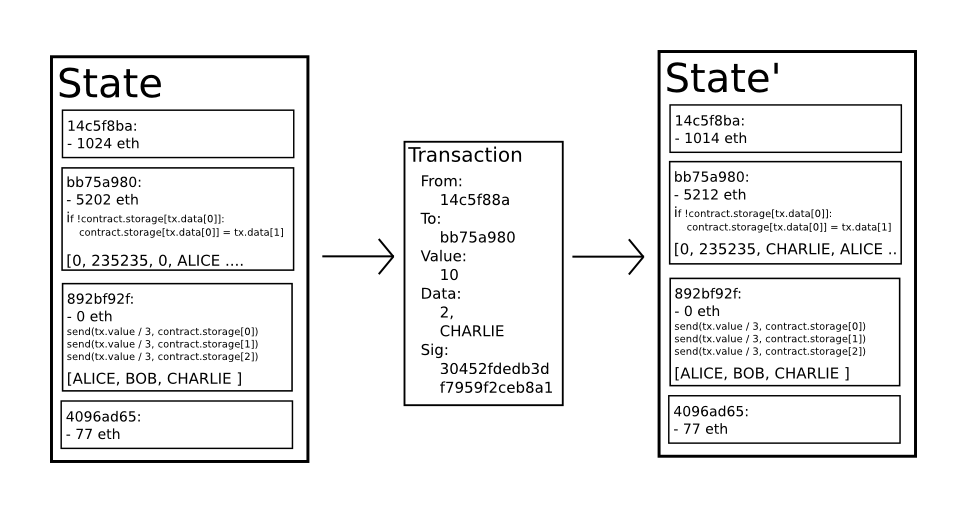
\includegraphics[scale=0.5]{ethertransition.png}
\end{center}
This function, \texttt{APPLY(S,TX) -> S'} can be defined as follows:
\begin{enumerate}
    \item Check if the transaction is well-formed (i.e. has the right number of values), the signature is valid, and the nonce matches the nonce in the sender's account. If not, return an error.
    \item Calculate the transaction fee as STARTGAS * GASPRICE, and determine the sending address from the signature. Subtract the fee from the sender's account balance and increment the sender's nonce. If there is not enough balance to spend, return an error.
    \item Initialize GAS = STARTGAS, and take off a certain quantity of gas per byte to pay for the bytes in the transaction.
    \item Transfer the transaction value from the sender's account to the receiving account. If the receiving account does not yet exist, create it. If the receiving account is a contract, run the contract's code either to completion or until the execution runs out of gas.
    \item If the value transfer failed because the sender did not have enough money, or the code execution ran out of gas, revert all state changes except the payment of the fees, and add the fees to the miner's account.
    \item Otherwise, refund the fees for all remaining gas to the sender, and send the fees paid for gas consumed to the miner.
\end{enumerate}

\section{Ethereum Smart Contracts}
A smart contract \cite{clack2016smart} is a computer protocol intended to digitally facilitate, verify, or enforce the negotiation or performance of a contract. Smart contracts allow the performance of credible transactions without third parties. These transactions are trackable and irreversible. Smart contracts were first proposed by Nick Szabo, who coined the term, in 1994.

There are, basing on applications, four types of smart conntract:
\begin{itemize}
    \item \textit{Smart Legal Contract}: smart contract combined with legal contract templates;
    \item \textit{Decentralized Autonomous Organizations (DAO)}: multiple smart contracts combined with governance mechanism;
    \item \textit{Distributet Applications (DApps)}: Combination of smart contract codes;
    \item \textit{Smart Contracting Devices}: combined with devices (IoT).
\end{itemize}

Proponents of smart contracts claim that many kinds of contractual clauses may be made partially or fully self-executing, self-enforcing, or both. The aim of smart contracts is to provide security that is superior to traditional contract law and to reduce other transaction costs associated with contracting. Various cryptocurrencies have implemented types of smart contracts. 

A smart contract can be deployed using three different languages:
\begin{itemize}
    \item \textit{Solidity}: A Javascript-like Object Oriented language;
    \item \textit{Serpent}: A Python-like Object Oriented language;
    \item \textit{LLL (Low-level Lisp-like Language)}: A Lisp-like Functional language.
\end{itemize}


\section{Applications in Token Systems}
On-blockchain token systems have many applications ranging from sub-currencies representing assets such as USD or gold to company stocks, individual tokens representing smart property, secure unforgeable coupons, and even token systems with no ties to conventional value at all, used as point systems for incentivization. \newline
Token systems are surprisingly easy to implement in Ethereum. The key point to understand is that all a currency, or token system, fundamentally is a database with one operation: subtract \texttt{X} units from \texttt{A} and give \texttt{X} units to \texttt{B}, with the proviso that 
\begin{enumerate}
    \item \texttt{A} had at least \texttt{X} units before the transaction;
    \item The transaction is approved by \texttt{A}.
\end{enumerate}

All that it takes to implement a token system is to implement this logic into a contract.
The basic code for implementing a token system in Serpent looks as follows:
\begin{lstlisting}[language=Python]
def send(to, value):
    if self.storage[msg.sender] >= value:
        self.storage[msg.sender] = self.storage[msg.sender] - value
        self.storage[to] = self.storage[to] + value
\end{lstlisting}

Theoretically, Ethereum-based token systems acting as sub-currencies can potentially include another important feature that on-chain Bitcoin-based meta-currencies lack: the ability to pay transaction fees directly in that currency. The way this would be implemented is that the contract would maintain an ether balance with which it would refund ether used to pay fees to the sender, and it would refill this balance by collecting the internal currency units that it takes in fees and reselling them in a constant running auction. Users would thus need to "activate" their accounts with ether, but once the ether is there it would be reusable because the contract would refund it each time.